\documentclass[lang=en,color=green]{elegantbook}
\title{Pragmatic Node.js development}
\subtitle{Primer in Nest.js}

\author{Zlatibor Zed Veljkovic}
\date{June 5, 2022}
\version{0.1}
\bioinfo{bioinfo 1}{bioinfo 2} 

\extrainfo{Some extra info}

\setcounter{tocdepth}{3}

\logo{cule.jpg}
\cover{cover.jpg}
 
% 本文档命令
\usepackage{array}
\usepackage{enumitem}
\newcommand{\ccr}[1]{\makecell{{\color{#1}\rule{1cm}{1cm}}}}

% 修改标题页的橙色带 
% \definecolor{customcolor}{RGB}{32,178,170}
% \colorlet{coverlinecolor}{customcolor}

\begin{document}

\maketitle
\frontmatter

\tableofcontents

\mainmatter

\chapter{Developer tools}

Since ancient times, mankind has constantly spent effort to create new or to improve existing tools. 
Even now, after thousands and thousands of years we are doing the same. 
We are making new tools that will make us more efficient or at least to do our tasks easier.
In software development there are so many tools available it is hard to choose which set should be used. Next sections will give simple overview of most prominent tools for each section. 


\section{Command line interfaces}
Commad line interfaces (CLI) are programs that use textual interface and allow you to interact with it. 
Every operating system comes with one or more of these, Windows has Command Prompt (aka cmd.exe) and Power Shell,
Linux has sh and bash with many alternatives (commonly known as shell), and Mac OS has Terminal.app. 
One issue that novice developers struggle is that when someone tells you to “open the terminal”,
they mean one for your system. 

Before mentioned apps are the ones that allow you to execute some commands or run different programs.
There are also some CLI that is specifically built for one purpose. 
One example would be Nest.js CLI which allows you to quickly create new projects,
 update dependencies or start the Nest app. 

\subsection{Command prompt} 
Command prompt comes preinstalled on Windows systems.
It supports batch scripts and usually the file is with .bat extension.

\noindent\begin{minipage}[t]{0.5\textwidth}%
    \centering{Pros} 
    \begin{itemize}[leftmargin=*]
        \item Available on all Windows systems
        \item Allows executing programs in current directory without  \lstinline{.\}  prefix
    \end{itemize}
\end{minipage}%
\begin{minipage}[t]{0.5\textwidth}%
    \centering{Cons} 
    \begin{itemize}[leftmargin=*]
        \item Batch scripting language is really outdated and hard to write more complex stuff
    \end{itemize}
\end{minipage}%

\begin{figure}[htbp]
    \centering
    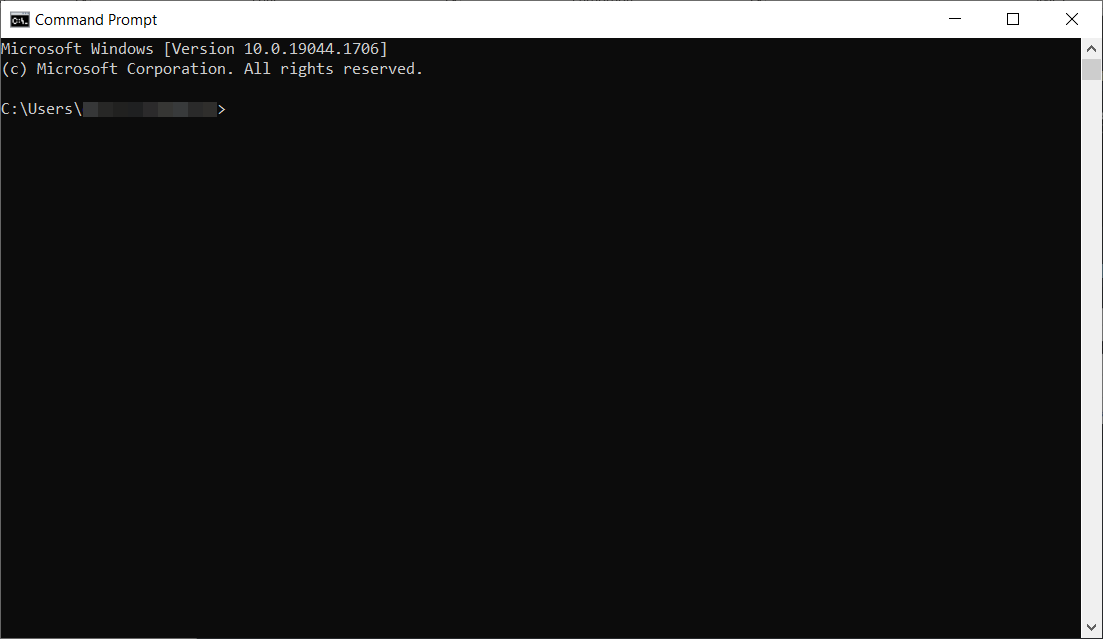
\includegraphics[width=0.6\textwidth]{images/command-prompt.png}
    \caption{Command Prompt\label{fig:Command Prompt}}
\end{figure}

Reference for available Command Prompt commands can be found at \href{https://docs.microsoft.com/en-us/windows-server/administration/windows-commands/windows-commands}{Windows Commands}

\subsection{PowerShell} 
Another shell for Windows systems is called PowerShell and it is available from
Windows 7 or later operating systems. Open source version PowerShell Core was released in 2016 and  
it is based on .Net Core which also made it cross-platform. It has better integration
with various functionalities available in Windows so it is prefreed choice over Command Prompt
when working with system administration. For developer work it might be an overkill.


\noindent\begin{minipage}[t]{0.5\textwidth}%
    \centering{Pros} 
    \begin{itemize}[leftmargin=*]
        \item Available on all Windows systems
        \item Better integration with Windows functionalities
    \end{itemize}
\end{minipage}%
\begin{minipage}[t]{0.5\textwidth}%
    \centering{Cons} 
    \begin{itemize}[leftmargin=*]
        \item  Does not allow executing programs in 
        current directory without  \lstinline{.\} prefix
    \end{itemize}
\end{minipage}%

\begin{figure}[htbp]
    \centering
    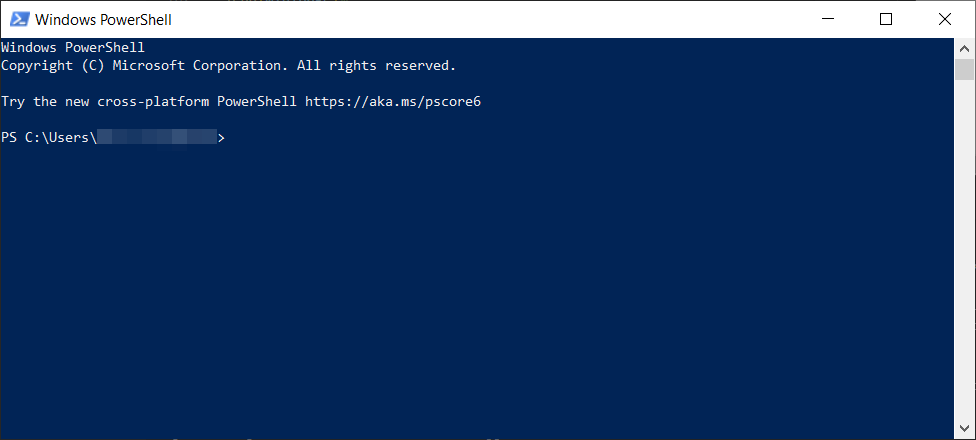
\includegraphics[width=0.6\textwidth]{images/powershell.png}
    \caption{PowerShell\label{fig:PowerShell}}
\end{figure}
ffhgf

\end{document}
